\FloatBarrier

\begin{figure}[h!]
	\centering
	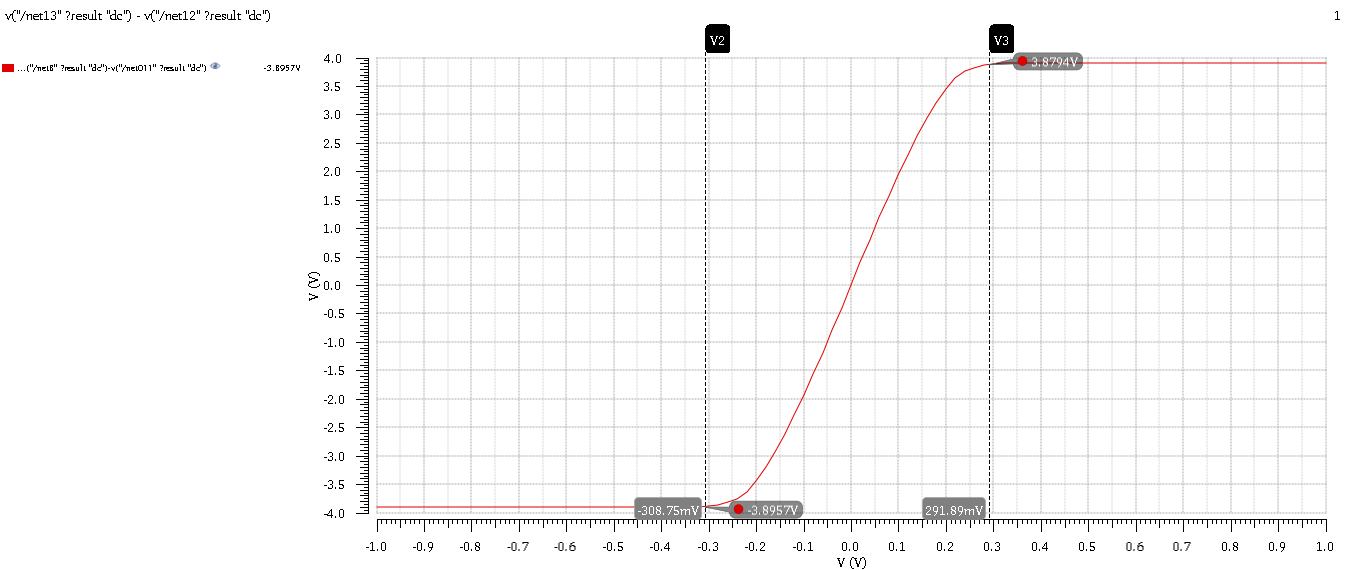
\includegraphics[scale=0.75]{../images/sim2_sweep.PNG}
	\caption{Simulation 2 Sweep - $V_{out,dm}$ versus $V_{in,dm}$}
	\label{fig:sim2_sweep}
\end{figure}

\FloatBarrier

Table (\ref{tab:sim2_sat}) contains the ranges of input and output differential-mode values for which the transistors are biased in saturation.

\FloatBarrier

\begin{table}[h!]
	\centering
	\caption{Conditions for All Transistors to be in Saturation}
	\label{tab:sim2_sat}
	\csvautotabular{../tables/sim2_sat.csv}
\end{table}

\FloatBarrier

The differential-mode gain can be acquired by computing the slope near $V_{in,dm} = 0$\si{\volt}.
Table (\ref{tab:sim2_gain}) contains these values.
The theoretical prediction is very close to the simulation result.

\FloatBarrier

\begin{table}[h!]
	\centering
	\caption{Simulation versus Theoretical Differential-Mode Gain}
	\label{tab:sim2_gain}
	\csvautotabular{../tables/sim2_gain.csv}
\end{table}

\FloatBarrier
